\documentclass[12pt]{article}

\usepackage{sbc-template}

\usepackage{graphicx,url}

\usepackage[brazil]{babel}
\usepackage[utf8]{inputenc}
\usepackage{comment}
\usepackage[T1]{fontenc}


\sloppy

\title{Experimento de algoritmo para economia de energia no\\
 escalonamento de workflows com Eucalyptus}

\author{Luís Filipe Resende Vilela\inst{1}, Victor Cotrim de Lima\inst{1}}

\address{Faculdade do Gama (FGA) -- Universidade de Brasília
  (UnB)\\
  Área Especial, Projeção A, UnB -- 72.444-240 -- Setor Leste -- Gama -- DF -- Brasil
}

\begin{document}

\maketitle

\begin{abstract}
  This article have the purpose to realize an experiment, previusly maked in article \cite{elaine_et_al:14}, using another IaaS tool. This experiment have only elucidative objective with purpose of learn in matter Cloud Computing at University of Brasilia, campus Gama.
\end{abstract}

\begin{resumo}
  Este artigo tem como intuito realizar o experimento consolidade no artigo \cite{elaine_et_al:14}, utilizando de outra ferramenta do tipo Infra-estrutura como um Serviço\footnote{\textit{IaaS}}. Este exeperimento tem caráter elucidativo, utilizando somente como forma de aprendizagem para a matéria de Computação em Núvem da Universidade de Brasília, campus Gama.

\end{resumo}


\section{Introdução}

Nuvem nos dias atuais

graças a virtualização e expansibilidade, cpu memória

autonômica, elasticidade

Segundo \cite{coutinho_et_al:14} foi realizado um experimento, que criou uma instância de aglomerado com 26.496 núcleos, usando máquinas do tipo \textit{c3.8xlarge} da Amazon EC2, foi observado que o desempenho dessa instância foi equivalente ao de uma máquina com 484,2 TeraFLOPS, o que comprova o fornecimento de um ambiente de alto desempenho gerado pela Computação em Nuvem.

O artigo está estruturado da seguinte forma:
\begin{itemize}
  \item Seção 2 será descrito o ambiente para replicação do artigo \cite{coutinho_et_al:14}.
  \item Seção 3 será descrito um paralelo entre: como o artigo propôs a implementação do mesmo e como o experimento deste artigo foi realizado.
  \item Seção 4 será descrito as dificuldades, problemas e soluções em relação ao desenvolvimento da replicação dos resultados do artigo.
  \item Seção 5 será descrito os resultados.
\end{itemize}

\section{Ambiente}

No artigo analisado foi utilizado a ferramenta \textit{OpenNebula} e a arquitetura \textit{FairCPU} para uma estratégia baseada em balanceadores de carga (elasticidade horizontal). O OpenNebula é um conjunto de ferramentas de IaaS open source, que pode ser utilizado para geração de uma nuvem privada. No que se refere a nuvem privada, sua infraestrutura opera exclusivamente para uma única organização ou usuário, seja ela gerida internamente ou por um terceiro, e hospedada internamente ou externamente.

O \textit{FairCPU} é uma arquitetura para provisionamento de máquinas virtuais utilizando
características de processamento~\cite{faircpu:12}. \textit{FairCPU} utiliza unidades de processamento (UPs) para alocar recursos de CPU para as MVs\footnote{Máquinas Virtuais}, de forma a garantir que o desempenho da MV seja homogêneo, independente da MF subjacente. A UP e a abstração utilizada para representar o poder de processamento de MFs e MVs, e deve ter um valor constante e conhecido (ex. GFLOPS, MIPS, ou outra métrica) e substitui o valor bruto da quantidade de CPUs, que é o parâmetro utilizado na maioria dos middleware e atuais provedores de IaaS no momento de alocar as MVs.

Essa ferramenta foi utilizada no artigo \cite{coutinho_et_al:14} proposto por possibilitar a simulação em nuvens computacionais para avaliar em conjunto ao \textit{FairCPU} o comportamento do ambiente diante de cargas de trabalho, e como se comportam de maneira autonômica para adaptação a variações de demanda (elasticidade) e manutenção do SLA.

Nesse artigo foram utilizadas as ferramentas \textit{CloudStack}, na versão 4.4, para simulação e geração de nuvens computacionais e o \textit{VMWare}\footnote{a.k.a Virtual Machine Ware} para simulação de virtualização. O \textit{CloudStack}
é uma ferramente de software de código aberto para computação em nuvem que implementa o que é comumente referido como infraestrutura como serviço (IaaS), que são sistemas que dão aos usuários a capacidade de executar e controlar instâncias de máquinas virtuais inteiras implantados através de uma variedade de recursos físicos~\cite{nurmi_2009}. 

A \textit{VMWare} foi utilizada para a criação de uma máquina virtual do sistema operacional Ubunto Server 14.04.1 para replicação do experimento ocorrido no \cite{elaine_et_al:14}. O conceito de máquina virtual é definido pela IBM como: uma cópia do hardware físico da máquina totalmente protegido e isolado. Assim, cada usuário de uma máquina virtual possui a ilusão de ter uma máquina física dedicada. Os desenvolvedores de software também podem escrever e testar programas sem o medo de deixar que a máquina física
não funcione e afete outros usuários. \cite{sugerman2001virtualizing}.

\section{Metodologia}

O objetivo deste artigo, é o da replicação do experimento feito em \cite{coutinho_et_al:14}. Os problemas encontrados no decorrer do experimento foram devidamente citados na seção \ref{sec:dificuldades}.

Para iniciar o experimento de replicação, inicialmente foi feita o levantamento de ambiente, que consistiu basicamente do download do \textit{hipervisor}\footnote{Camada de software localizada entre a camada de hardware e o sistema operacional\cite{dev_midia}} de simulação de virtualização \textit{VMWare}\footnote{a.k.a Virtual Machine Ware} e do download da imagem virtual do sistema operacional \textit{Ubunto Server} onde ficará o \textit{CloudStack}. Esta imagem virtual contém uma imagem do sistema operacional Ubunto 14.04.1 onde o \textit{CloudStack} será posteriormente instalado. Após algumas configuraçoes na máquina virtual, o CloudStack poderá ser iniciado pelo brownser. 

Após efetuado login, é necessário configurar o \textit{Zone}, \textit{Pod}, \textit{Cluster}, \textit{Storage} e por fim o \textit{Host}.

No artigo alvo, foi fornecido um repositório aberto no \textit{GitHub}, com o código do artigo completamente implementado. Uma forma de avaliar o que o artigo propõe é simplesmente executar o que já foi implementado e comparar os resultados da execução com o do artigo alvo.

Foi utilizado o algoritmo implementado do código recuperado do repositório indicado no artigo alvo.

Para a utilização deste algoritmo houve uma substituição do código implementado no código do \textit{Eucalyptus}.

O último passo foi lançar as instâncias de máquinas virtuais para simular o experimento. 

\section{Dificuldades}
\label{sec:dificuldades}

Este artigo foi feito baseado na atividade de refazer o experimento no artigo \cite{coutinho_et_al:14} utilizando de outra tecnologia que não fosse usada no artigo alvo. O artigo alvo usa a ferramenta \textit{OpenNebula}. Já o experimento de replicação está usando o \textit{ClouStack}. Este experimento foi feito para a matéria de Computação em Nuvem da Faculdade do Gama.

Baseado neste fato, alguns problemas relacionados a esta adaptação foram encontrados.

\begin{enumerate}

  \item Instalação da ferramenta CloudStack

  \begin{itemize}
    \item Problema: Foi feita a escolha de instalar o CloudStack em uma máquina virtual com o Sistema Operacional Mint 17.1, porém não existe, atualmente, as dependências que necessitam ser instaladas.
    \item Solução: Houve a troca do Sistema Operacional para Ubunto Server 14.04.1.
  \end{itemize}

  \item Simulação de máquinas virtuais
  \begin{itemize}
    \item Problema: O CloudStack não faz simulação, somente a virtualização de ambiente como nuvem.
    \item Solução: Utilização de máquinas virtuais em baixa quantidade.
  \end{itemize}

  \item Simulação da quantidade requerida de máquinas virtuais
  \begin{itemize}
    \item Problema: O computador utilizado como Nó de controle para o CloudStack, não tem poder computacional para virtualização da quantidade mínima de máquinas requerida pelo artigo alvo.
    \item Solução: Utilização de uma quantidade mínima para simulação
  \end{itemize}

  \item Criação de um Host
  \begin{itemize}
    \item Problema: A criação do Host não foi com sucesso.
    \item Solução: Tentar procurar como corrigir o problema e criar um Host. Porém a procura não foi bem sucedida, pois chegou-se que o computador não possui poder computacional suficiente para criar um Host.
  \end{itemize}



\end{enumerate}


\begin{comment}

  \item Instalação da ferramenta CloudStack
  \begin{itemize}
    \item Problema:
    \item Solução:
  \end{itemize}


\end{comment}

\section{Resultados}

Foi observado que ao se replicar o experimento com uma ferramenta de IaaS diferente da utilizada no artigo alvo, algumas complicações foram observadas. Desde o levantamento do ambiente até a tentativa de levantamento de instâncias de máquinas virtuais.

Como resultado principal, não foi possível simular os testes do artigo alvo no experimento de replicação.

E como um forte conclusão, foi percebido que a utilização da ferramenta \textit{CloudStack}, para simulação de Hosts, não é desejavel com a privação de poder computacional. Pois a ferramenta \textit{CloudStack} não , e para replicar o experimento seria necessário um grande poder computacional para instanciar as máquinas e configura-las de forma correta.




% \section{General Information}
%
%
% All full papers and posters (short papers) submitted to some SBC conference,
% including any supporting documents, should be written in English or in
% Portuguese. The format paper should be A4 with single column, 3.5 cm for upper
% margin, 2.5 cm for bottom margin and 3.0 cm for lateral margins, without
% headers or footers. The main font must be Times, 12 point nominal size, with 6
% points of space before each paragraph. Page numbers must be suppressed.
%
% Full papers must respect the page limits defined by the conference.
% Conferences that publish just abstracts ask for \textbf{one}-page texts.
%
% \section{First Page} \label{sec:firstpage}
%
% The first page must display the paper title, the name and address of the
% authors, the abstract in English and ``resumo'' in Portuguese (``resumos'' are
% required only for papers written in Portuguese). The title must be centered
% over the whole page, in 16 point boldface font and with 12 points of space
% before itself. Author names must be centered in 12 point font, bold, all of
% them disposed in the same line, separated by commas and with 12 points of
% space after the title. Addresses must be centered in 12 point font, also with
% 12 points of space after the authors' names. E-mail addresses should be
% written using font Courier New, 10 point nominal size, with 6 points of space
% before and 6 points of space after.
%
% The abstract and ``resumo'' (if is the case) must be in 12 point Times font,
% indented 0.8cm on both sides. The word \textbf{Abstract} and \textbf{Resumo},
% should be written in boldface and must precede the text.
%
% \section{CD-ROMs and Printed Proceedings}
%
% In some conferences, the papers are published on CD-ROM while only the
% abstract is published in the printed Proceedings. In this case, authors are
% invited to prepare two final versions of the paper. One, complete, to be
% published on the CD and the other, containing only the first page, with
% abstract and ``resumo'' (for papers in Portuguese).
%
% \section{Sections and Paragraphs}
%
% Section titles must be in boldface, 13pt, flush left. There should be an extra
% 12 pt of space before each title. Section numbering is optional. The first
% paragraph of each section should not be indented, while the first lines of
% subsequent paragraphs should be indented by 1.27 cm.
%
% \subsection{Subsections}
%
% The subsection titles must be in boldface, 12pt, flush left.
%
% \section{Figures and Captions}\label{sec:figs}
%
%
% Figure and table captions should be centered if less than one line
% (Figure~\ref{fig:exampleFig1}), otherwise justified and indented by 0.8cm on
% both margins, as shown in Figure~\ref{fig:exampleFig2}. The caption font must
% be Helvetica, 10 point, boldface, with 6 points of space before and after each
% caption.
%
% \begin{figure}[ht]
% \centering
% 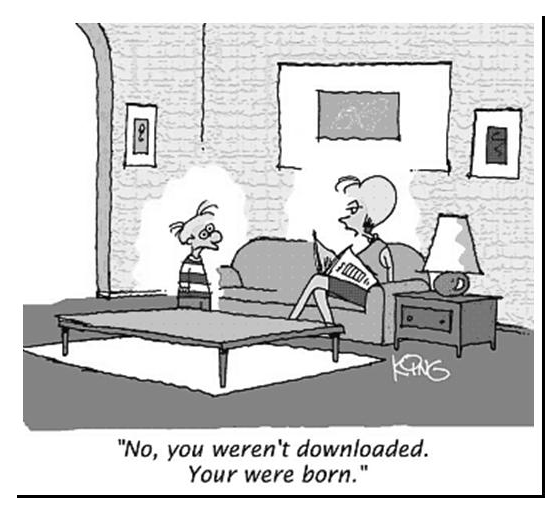
\includegraphics[width=.5\textwidth]{fig1.eps}
% \caption{A typical figure}
% \label{fig:exampleFig1}
% \end{figure}
%
% \begin{figure}[ht]
% \centering
% 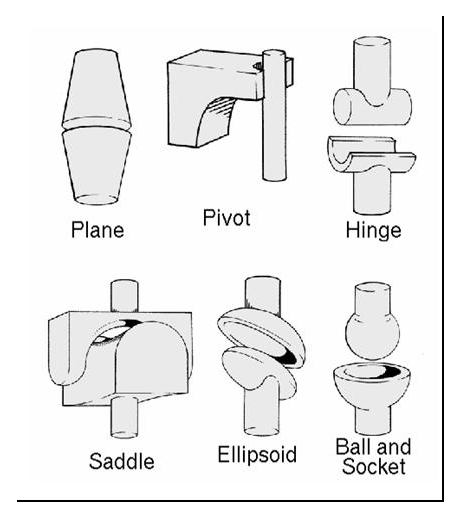
\includegraphics[width=.3\textwidth]{fig2.eps}
% \caption{This figure is an example of a figure caption taking more than one
%   line and justified considering margins mentioned in Section~\ref{sec:figs}.}
% \label{fig:exampleFig2}
% \end{figure}
%
% In tables, try to avoid the use of colored or shaded backgrounds, and avoid
% thick, doubled, or unnecessary framing lines. When reporting empirical data,
% do not use more decimal digits than warranted by their precision and
% reproducibility. Table caption must be placed before the table (see Table 1)
% and the font used must also be Helvetica, 10 point, boldface, with 6 points of
% space before and after each caption.
%
% \begin{table}[ht]
% \centering
% \caption{Variables to be considered on the evaluation of interaction
%   techniques}
% \label{tab:exTable1}
% 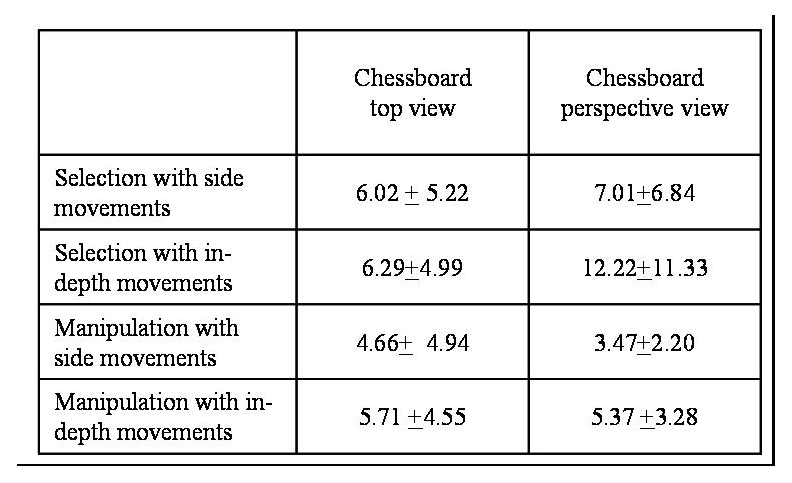
\includegraphics[width=.7\textwidth]{table.eps}
% \end{table}
%
% \section{Images}
%
% All images and illustrations should be in black-and-white, or gray tones,
% excepting for the papers that will be electronically available (on CD-ROMs,
% internet, etc.). The image resolution on paper should be about 600 dpi for
% black-and-white images, and 150-300 dpi for grayscale images.  Do not include
% images with excessive resolution, as they may take hours to print, without any
% visible difference in the result.
%
% \section{References}
%
% Bibliographic references must be unambiguous and uniform.  We recommend giving
% the author names references in brackets, e.g. \cite{knuth:84},
% \cite{boulic:91}, and \cite{smith:99}.
%
% The references must be listed using 12 point font size, with 6 points of space
% before each reference. The first line of each reference should not be
% indented, while the subsequent should be indented by 0.5 cm.

\bibliographystyle{sbc}
\bibliography{bibliografia}

\end{document}
